\section{Method}
\subsection{Silicon Chips}
\subsubsection{Glassgow}
\begingroup
    \centering  
    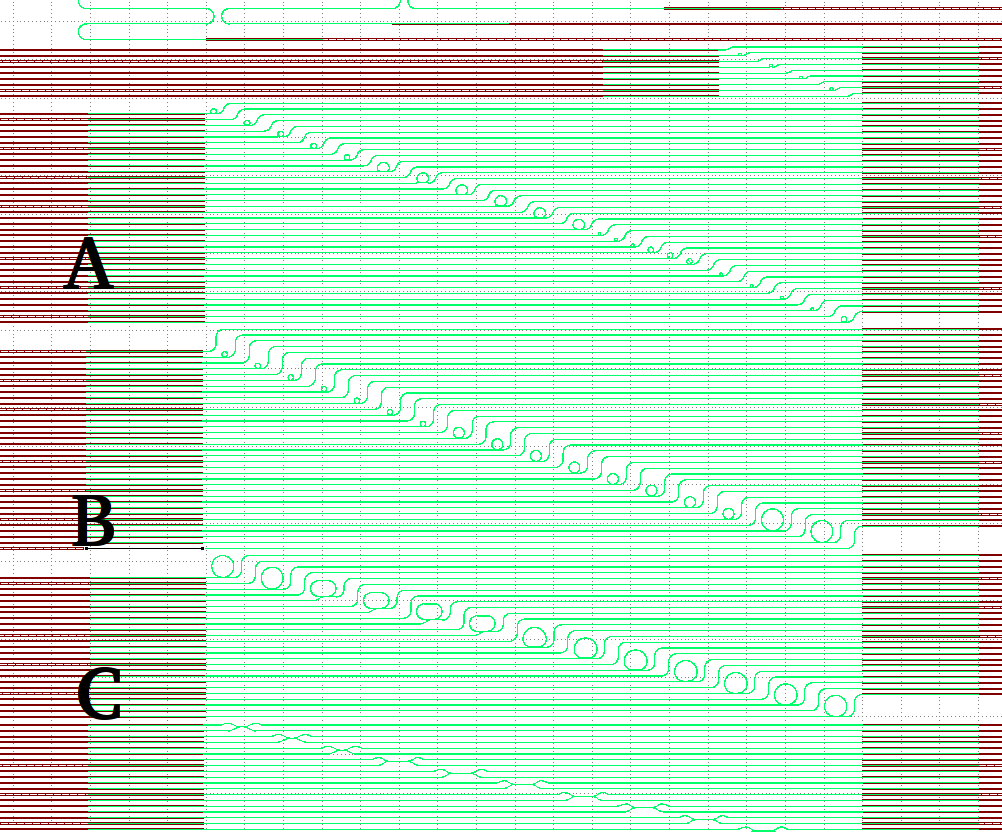
\includegraphics[width=10cm]{img/results/glassgowChipNumbering.png}
    \captionof{figure}{Glassgow test structure chip}
     \vspace{3pt} \label{crossCompare}
\endgroup
\subsubsection{Toshiba}
\begingroup
    \centering  
    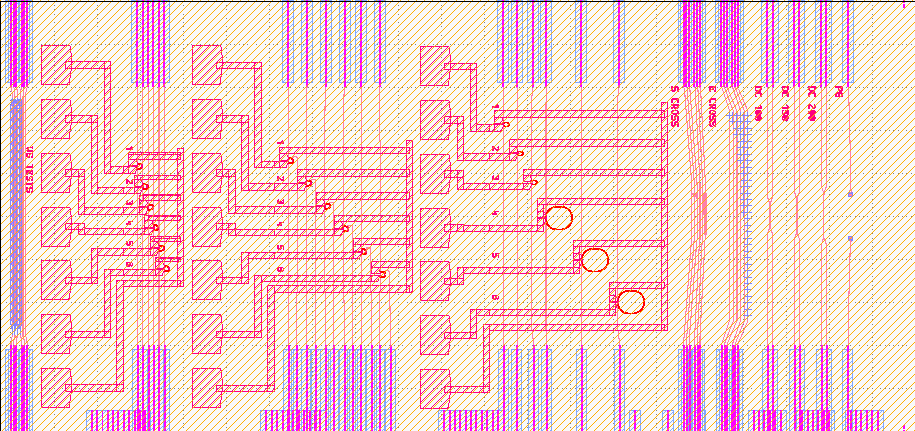
\includegraphics[width=10cm]{img/results/toshiba.png}
    \captionof{figure}{Glassgow test structure chip}
     \vspace{3pt} \label{crossCompare}
\endgroup
\subsubsection{a-Si}
\begingroup
    \centering  
    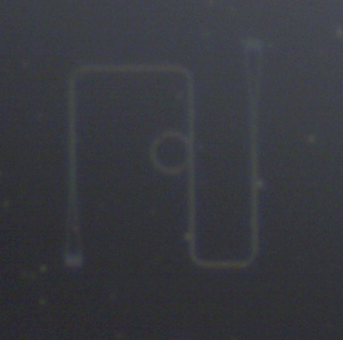
\includegraphics[width=10cm]{img/results/chipPictures/exampleASIRing.png}
    \captionof{figure}{Glassgow test structure chip}
     \vspace{3pt} \label{crossCompare}
\endgroup
\subsection{Coupling}
% Side/Vertical coupling
% Coupling loss
% Blowing up chips -> tempted to add this as a complaint
%	Particularly on glassgow chip
% Temperature tuning
\subsection{Joint Spectrum}
% OSA Resolution discussion might be important. Because I think it might have skrewed me over somewhat.
% Filtering
\subsection{What experiments can be done?}
Assuming from the above that the procedure for collecting the JSI is fixed and fully understood the question that now needs to be answered is: what parameters can be reliably varied to change the JSI?
One that we pursue and that forms the main part of this work is varying the power of the pump laser injected into the ring. This is of interest as it may 
\subsection{$g^{(2)}(0)$}
% Breif description of how this works.
\subsection{Analysing Data}
% NOISE
% NORALISATION
% SPM
% RING DEFORMATION

% I want to really discuss what we can hope to keep constant and what we can vary. Where you need to really do som engineering to get insights.